\documentclass[a4paper]{ltjsarticle}

\usepackage[margin=15mm]{geometry}

\usepackage{graphicx}

% \renewcommand{\baselinestrech}{0.8}

\begin{document}

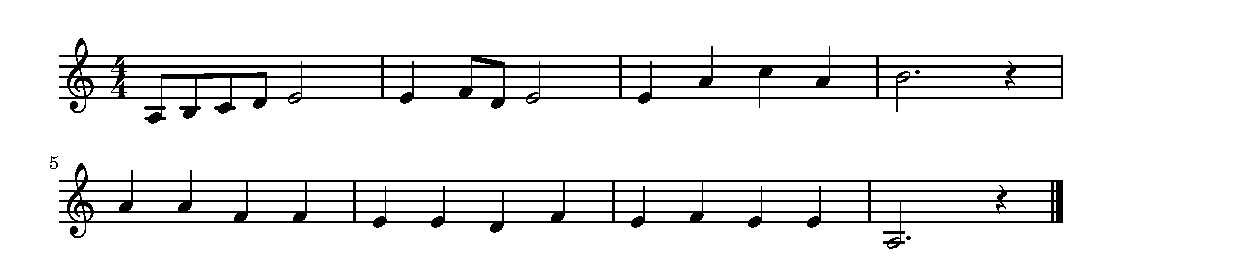
\includegraphics[clip]{akaikutsu_crop.pdf}

\vspace{-10mm} \hspace{10mm}
赤い靴(あかいくつはいてたおんなのこ)



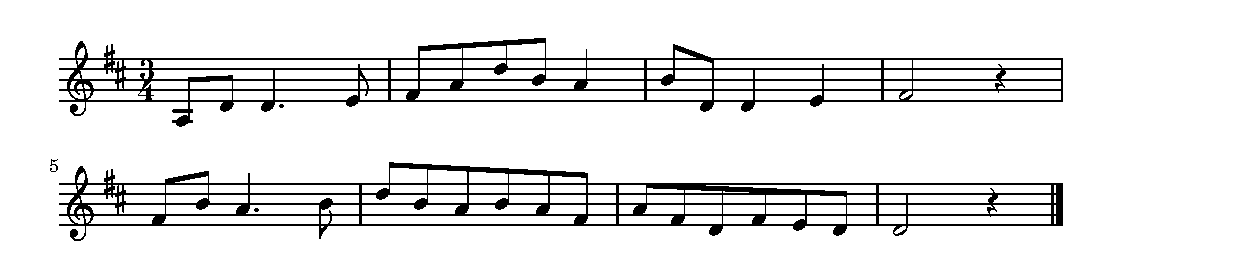
\includegraphics[clip]{akatonbo_crop.pdf}



\vspace{-10mm} \hspace{10mm}
赤とんぼ(ゆうやけこやけのあかとんぼ)




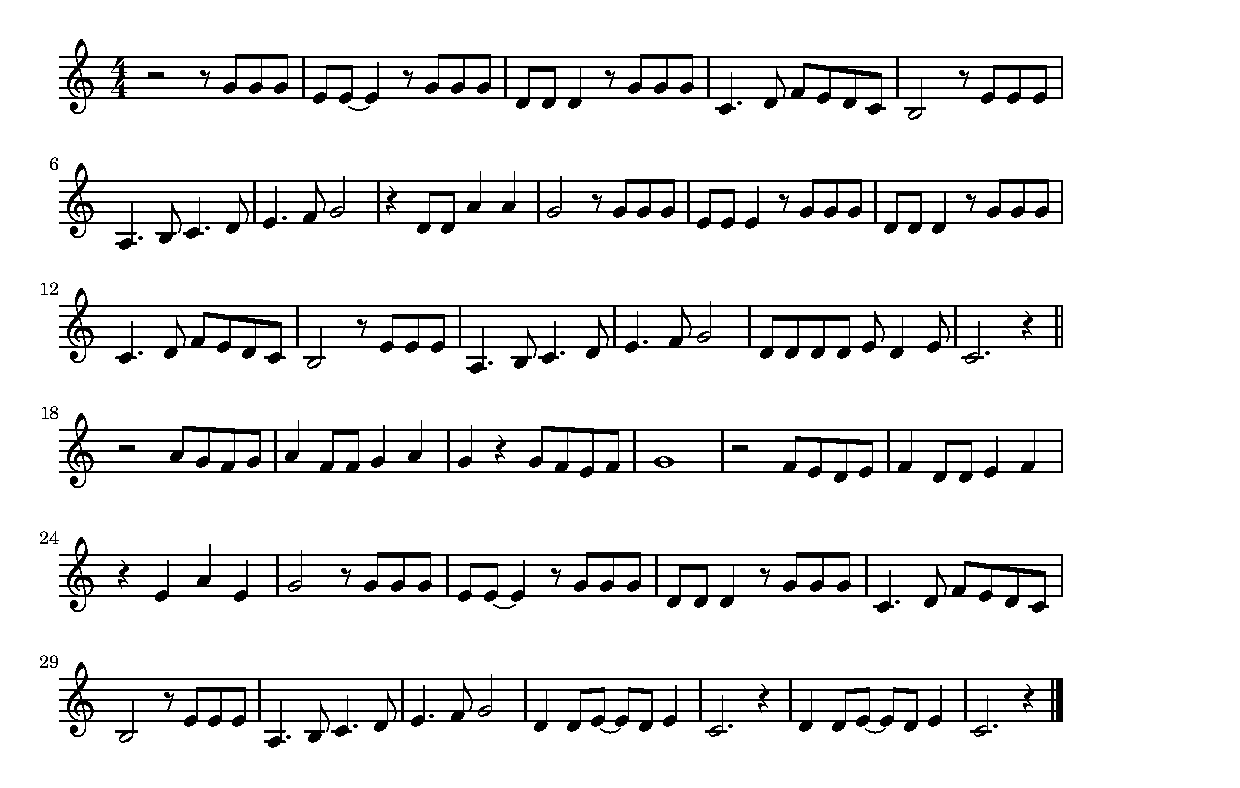
\includegraphics[clip]{amaironokami_crop.pdf}



\vspace{--10mm} \hspace{10mm}
亜麻色の髪の乙女(あまいろのながいかみをかぜが)



\end{document}